\documentclass[twocolumn]{article}
\usepackage{amsmath, amssymb, amsthm}
\usepackage{tikz}
\usetikzlibrary{arrows,decorations.markings}
\usepackage[T1]{fontenc}
\usepackage{mathptmx}
\usepackage{stix}
\usepackage{textcomp}
%\usepackage{simpsons}
\usepackage{multicol}
\usepackage[makeroom]{cancel}
\usepackage[utf8]{inputenc}
\usepackage{pdfpages}
\usepackage{geometry}
 \geometry{
	 a4paper,
	 left=10mm,
	 right=10mm,
	 top=10mm,
	 bottom=20mm,
	 }
\usepackage{hyperref}
\begin{document}
\Large
\begin{equation*}
	\frac{d}{dt}\Bigg{\{} U + m \Bigg{(}\frac{c^2}{2}+gz\Bigg{)}\Bigg{\}} 
	= 
	\sum_{j}{\Bigg{[}\dot{m}_j\Bigg{(}h+\frac{c^2}{2}+gz\Bigg{)}_j \Bigg{]}}  
	+ 
	\sum_{l}^{} \Big(\dot{Q}_t\Big)_l 
	+ 
	\sum_{i}\Big(\dot{W}_t\Big)_i
	-
	p\frac{dV}{dt}
\end{equation*}
\normalsize
\section{Nomenklatur}


\begin{align*}
	\mathbf{An}		&=	\text{Anergie[J]} \\
	\mathbf{c_s}		&=	\text{Schallgeschwindigkeit[m/s]} \\
	\mathbf{c_p}		&=	\text{Spezifische Wärmekapazität dp = 0 [J/kg*K]} \\
	\mathbf{c_v}		&=	\text{Spezifische Wärmekapazität dv = 0 [J/kg*K]} \\
	\mathbf{E}		&=	\text{Energie[J]} \\
	\mathbf{Ex = -W_{ex}}	&=	\text{Exergie[J]} \\
	\mathbf{F}		&=	\text{Kraft[N]} \\
	\mathbf{F = U - TS}	&=	\text{Freie Energie[J]} \\
	\mathbf{f = u-Ts}	&=	\text{Spezifische freie Energie[J/kg]} \\
	\mathbf{f}		&=	\text{Fugazität[Pa]} \\
	\mathbf{G = H -TS}	&=	\text{Freie Enthalpie[J]} \\
	\mathbf{g = h -Ts}	&=	\text{Spezifische freie Enthalpie[J/kg]} \\
	\mathbf{g}		&=	\text{Erdbeschleunigung[m/s²]} \\
	\mathbf{H = U+pV}	&=	\text{Enthalpie[J]} \\
	\mathbf{h = u + pv}	&=	\text{Spezifische Enthalpie[J/kg]} \\
	\mathbf{\Delta Hg}	&=	\text{Molare Reaktionsenthalpie} \\
	\mathbf{K}		&=	\text{Konstante des Massenwirkungsgesetztes[-]} \\
	\mathbf{M}		&=	\text{Molmasse[kg/mol]} \\
	\mathbf{\dot{m}}	&=	\text{Massestrom[kg/s]} \\
	\mathbf{m'}		&=	\text{Masse in der flüssigen Phase[kg]} \\
	\mathbf{m''}		&=	\text{Masse in der gasförmigen Phase[kg]} \\
	\mathbf{Ma=c/c_s}	&=	\text{Machzahl[-]} \\
	\mathbf{n=m/M}		&=	\text{Molzahl[mol]} \\
	\mathbf{n}		&=	\text{Polytropenexponent[-]} \\
	\mathbf{P_t}		&=	\text{technische Leistung[W]} \\
	\mathbf{Q}		&=	\text{Wärme[J]} \\
	\mathbf{\dot{Q}}	&=	\text{Wärmestrom[W]} \\
	\mathbf{q}		&=	\text{Spezifische Wärme[J/kg]} \\
	\mathbf{r}		&=	\text{Spezifische Verdampfungsenthalpie[J/kg]} \\
	\mathbf{R}		&=	\text{Gaskonstante[J/(kg K)]} \\
	\mathbf{R_m}		&=	\text{Universelle Gaskonstante[J/(mol K)]} \\
	\mathbf{S}		&=	\text{Entropie[J/K]} \\
	\mathbf{s}		&=	\text{Spezifische Entropie[J/(kg K)]} \\
	\mathbf{T}		&=	\text{Temperatur[K]} \\
	\mathbf{t}		&=	\text{Zeit[s]} \\
	\mathbf{t}		&=	\text{Temperatur[\textcelsius{}]} \\
	\mathbf{T}		&=	\text{Sättigungstemperatur[K]} \\
	\mathbf{U}		&=	\text{Innere Energie[J]} \\
	\mathbf{u}		&=	\text{Spezifische innere Energie [J/kg]} \\
\end{align*}
\\\\\\\\
\begin{align*}
	\mathbf{V}		&=	\text{Volumen[m³]} \\
	\mathbf{v}		&=	\text{Spezifisches Volumen[m³/kg]} \\
	\mathbf{V_m}		&=	\text{Molares Volumen[m³/mol]} \\
	\mathbf{W}		&=	\text{Arbeit[J]} \\
	\mathbf{w}		&=	\text{Spezifische Arbeit[J/kg]} \\
	\mathbf{W_V}		&=	\text{Volumenänderungsarbeit[J]} \\
	\mathbf{W_{el}}		&=	\text{Elektrische Arbeit[J]} \\
	\mathbf{W_w}		&=	\text{Wellenarbeit[J]} \\
	\mathbf{W_{diss}}	&=	\text{Dissipationsarbeit[J]} \\
	\mathbf{W_t}		&=	\text{Technische Arbeit[J]} \\
	\mathbf{W_{Virrev}}	&=	\text{Arbeitsverlust durch Irreversibilität[J]} \\
	\mathbf{x}=\frac{m''}{m'+m''}		&=	\text{Dampfanteil[-]} \\
	\mathbf{x}=\frac{m_{H_2O}}{m_L}		&=	\text{Wassergehalt} \\
	\mathbf{Z}		&=	\text{Allgemeine extensive Zustandsgrößen[Z]} \\
	\mathbf{z}		&=	\text{Allgemeine } \\
	\mathbf{\beta}		&=	\text{Isobarer Ausdehnungskoeffizient[1/K]} \\
	\mathbf{\gamma}		&=	\text{Isochorer Spannungskoeffizeint[1/K]} \\
	\mathbf{\delta_T}	&=	\text{Isothermer Drosselkoeffizient[m³/kg]} \\
	\mathbf{\delta_h}	&=	\text{Isenthalper Drosselkoeffizient[Ks²m/kg]} \\
	\mathbf{\varepsilon}	&=	\text{Leistungsziffer[-]} \\
	\mathbf{\varepsilon}	&=	\text{Verdichtungsverhältnis[-]} \\
	\mathbf{\eta_{th}}	&=	\text{Thermischer Wirkungsgrad[-]} \\
	\mathbf{\eta_{mech}}	&=	\text{Mechanischer Wirkungsgrad[-]} \\
	\mathbf{\kappa}		&=	\text{Adiabaten- oder Isentropenexponent[-]} \\
	\mathbf{\lambda}	&=	\text{Reaktionslaufzahl[-]} \\
	\mathbf{\mu_i}		&=	\text{Chemisches Potential[J/mol]} \\
	\mathbf{\nu_i}		&=	\text{Stöchiometrische Koeffizienten[-]} \\
	\mathbf{\xi_i}		&=	\text{Masseanteil[-]} \\
	\mathbf{\pi}		&=	\text{Druckverhältnis[-]} \\
	\mathbf{\rho}		&=	\text{Dichte[kg/m³]} \\
	\mathbf{\tau}		&=	\text{Temperaturverhältnis[-]} \\
	\mathbf{\phi}		&=	\text{Relative Feuchte[-]} \\
	\mathbf{\phi}		&=	\text{Einspritzverhältnis[-]} \\
	\mathbf{\xi}		&=	\text{Isothermer Kompressibilitätskoeffizient[m²/N]} \\
	\mathbf{\Psi}		&=	\text{Dissipationsenergie[J]} \\
	\mathbf{\psi}		&=	\text{Spezifische Dissipationsenergie[J]} \\
	\mathbf{\psi}		&=	\text{Drucksteigerungsverhältnis[-]} \\
	\mathbf{\psi_i}		&=	\text{Molanteil[-]} \\
\end{align*}

\pagebreak

\section{Grundbegriffe}

Systeme 
\begin{itemize}

	\item Abgeschlossenes System - kein Stoff oder Energietransport
	\item Geschlossenes System - kein Stofftransport
	\item Offenes System - Stoff und Energietransport

\end{itemize}
Messgrößen
\begin{itemize}

	\item Prozessgrößen sind Wegabhängig (eg. Arbeit, Wärme)
	\item Zustandsgrößen sind Wegunabhängig (eg. Volumen, Druck)
	\item Intensive Zustandsgrößen sind unabhängig von der Größe des Systems (eg. Druck, Temperatur)
	\item Extensive Zustandsgrößen sind abhängig von der Größe des Systems (eg. Volumen, Masse)
\end{itemize}
Zustandsgleichungen
\begin{itemize}
	\item Thermisch $\rightarrow f(p, V, T) = 0$ 
	\item Kalorisch $\rightarrow f(U, V, T) = 0, \quad  U = U(V,T), \quad u = u(v,T)$ 
\end{itemize}

\section{Basisformeln}
\begin{align*}
	H &= U + pV  					\\
	dS&=\frac{\delta Q_{rev}}{T}			\\
	F &= U-TS					\\
	G &= H-TS 					\\
	W_{V,12} &= -\int_{1}^{2} p\; dV 		\\
	dS &= \frac{Q_{rev}}{T} + S_{prod}		\\
	\Psi_{12} &= \int_{1}^{2} T\; dS_{prod}		\\
	dU &= Tds -pdV + \underbrace{\sum_{k=1}^{K} \mu_k dn_k}_{\text{Für Mehrstoffsysteme}} \leftarrow \text{Gibbs} \\
	dG &= -SdT + Vdp +  \overbrace{\sum_{k=1}^{K} \mu_k dn_k} \qquad \leftarrow \text{Gibbs} \\
	dH &= TdS + Vdp + \sum_{k=1}^{K} \mu_k dn_k \qquad \leftarrow \text{Gibbs}\\
	dF &= -SdT -pdV + \sum_{k=1}^{K} \mu _k dn_k \qquad \leftarrow \text{Gibbs}\\
	dU &= \left(\frac{\partial U}{\partial S}\right)_{V,n_j} dS + \left(\frac{\partial U}{\partial V}\right)_{S,n_j} dV + \sum_{k=1}^{K} \left(\frac{\partial U}{\partial n_k}\right)_{S,V,n_j \neq n_k} dn_k  \\
	p_1 &= p_a  \frac{\varphi_1 - \varphi_a}{\varphi_b- \varphi_a}(p_b - p_a) \\
\end{align*}
\begin{equation*}
\overbrace{\frac{d}{dt}\Bigg{\{} U + m \Bigg{(}\frac{c^2}{2}+gz\Bigg{)}\Bigg{\}}}^{\text{Stationäres System -> 0}} = \overbrace{\sum_{j}{\Bigg{[}\dot{m}_j\Bigg{(}h+\frac{c^2}{2}+gz\Bigg{)}_j \Bigg{]}}}^{\text{Geschlossenes System -> 0}}  + \overbrace{\sum_{l}^{} \Big(\dot{Q}_t\Big)_l}^{\text{Kein Wärmestrom -> 0}} + \overbrace{\sum_{i}\Big(\dot{W}_t\Big)_i}^{\text{Keine Leistung -> 0}}- \overbrace{p\frac{dV}{dt}}^{\text{Keine Volumenänderung -> 0}}
\end{equation*}

\section{Maxwell}

\begin{align*}
	\left(\frac{\partial T}{\partial p}\right)_{S,n_j}
	&= \quad
	\left(\frac{\partial V}{\partial S}\right)_{p,n_j}
	\\\\
	\left(\frac{\partial S}{\partial V}\right)_{T,n_j}
	&= \quad
	\left(\frac{\partial p}{\partial T}\right)_{V,n_j}
	\\\\
	\left(\frac{\partial S}{\partial p}\right)_{T,n_j}
	&= -
	\left(\frac{\partial V}{\partial T}\right)_{p,n_j}
	\\\\
	\left(\frac{\partial \mu _i}{\partial T}\right)_{p,n_j}
	&= -
	\left(\frac{\partial S}{\partial n_i}\right)_{T,p,n_j \neq n_i}
	\\\\
	\left(\frac{\partial \mu_i}{\partial p}\right)_{T,n_j}
	&=
	\quad \left(\frac{\partial V}{\partial n_i}\right)_{T,p,n_j \neq n_i}
\end{align*}
\section{Guggenheim}
\Large
\begin{tabular}{llllll}
	-S  & U  & V&			&U &= U(S,V) \\ 
	H & $\neovsearrow$   &  F&       &H &= H(S,p) \\
	-p & G & T                &      &F &= F(T,V) \\
	 &  &                      &     &G &= G(T,p) \\
\end{tabular}
\normalsize
\break
\begin{align*}
	U &= U(S,V) \\
	H &= H(S,p) \\
	F &= F(T,V) \\
	G &= G(T,p) \\
\end{align*}
%\Bart


\section{Thermodynamische Beziehungen}
\begin{multicols}{2}

\begin{align*}
T &= \quad \left(\frac{\partial U}{\partial S}\right)_{V} \\
T &= \quad \left(\frac{\partial H}{\partial S}\right)_{p} \\
p &= - \left(\frac{\partial U}{\partial V}\right)_{S} \\
\mu &= \quad \left(\frac{\partial U}{\partial n}\right)_{S,V}  \\
\end{align*}
	\begin{align*}
		-S &= \left(\frac{\partial F}{\partial T}\right)_{V} \\
		-S &= \left(\frac{\partial G}{\partial T}\right)_{p} \\
		-p &= \left(\frac{\partial F}{\partial V}\right)_{T} \\
		V &= \left(\frac{\partial G}{\partial p}\right)_{T}  \\
	\end{align*}
\end{multicols}

\pagebreak
\section{Ideales Gas}
\begin{align*}
	&pV = mRT \\
	&pv = RT \\
	&pV = nR_mT \\
	&\beta = \frac{1}{T},\quad  \\
	&\gamma = \frac{1}{T},\quad 
	\chi = \frac{1}{p}, \quad \beta = p \gamma \chi, \quad  \\
	&R_m = 8,3143\left[\frac{kJ}{kmolK}\right], \quad 
	R = c_p - c_v \quad  \\
	&U - U_0 = mc_v(T-T_0) \\
	&H - H_0 = mc_p(T-T_0) \quad \leftarrow \text{Für $c_p$ und $c_v$ const.} \\
	&s - s_0 = R \ln \left(\frac{ v}{ v_0}\right)_{} + c_v \ln \left(\frac{ T}{ T_0}\right)_{} \\
	&\qquad \; = c_v \ln \left( \frac{p}{p_0} \right) + c_p \ln \left( \frac{v}{v_0} \right) \\
	&\qquad \; = c_p \ln \left( \frac{T}{T_0} \right) -R \ln \left( \frac{p}{p_0} \right) \\
	&\beta = \frac{1}{T} = \; \;\: \frac{1}{V}\left(\frac{\partial V}{\partial T}\right)_{p} =  \frac{1}{v}\left(\frac{\partial v}{\partial T}\right)_{p} =  - \frac{1}{\rho}\left(\frac{\partial \rho}{\partial T}\right)_{p}  \\
	&\gamma = \frac{1}{T} =  \; \;\; \frac{1}{p} \: \left(\frac{\partial p}{\partial T}\right)_{V} \\
	&\chi = \frac{1}{p} = - \frac{1}{V}\left(\frac{\partial V}{\partial p}\right)_{T}  = - \frac{1}{v}\left(\frac{\partial v}{\partial p}\right)_{T} \\
\end{align*}

\section{Van-der-Waals}
\begin{align*}
	&\left(p + \frac{a}{v^2}\right)(v-b) = RT \\
	&\left(\overline{p} + \frac{a}{\overline{v}^2}\right)(\overline{v}^3-b) = 8\overline{T} \\
	&\overline{p} = \frac{p}{p_K}, \quad \overline{v} = \frac{v}{v_K}, \quad \overline{T} = \frac{T}{T_K} \\
	&a=3p_Kv^2_K, \quad b =\frac{v_K}{3}, \quad \frac{p_Kv_K}{RT_K} = \frac{3}{8} \\
	&\beta = \frac{(v-b)Rv^2}{RTv^3 - 2a(v-b)^2} \\ 
	&\gamma = \frac{Rv^2}{RTv^2 - a(v-b)} \\
	&\chi = \frac{(v-b)^2v^2}{RTv^3 - 2a(v-b)^2} \\
	& du = \frac{a}{v^2}dv + c_v(T)dT \\
	&u-u_0 = \left( \frac{a}{v_0} - \frac{a}{v} \right) + \int_{T_0}^{T} c_v(\tilde{T})\; d\tilde{T} \\
	& u - u_0 = \left(\frac{a}{v_0} - \frac{a}{v} \right) + v_v(T-T_0) \leftarrow \text{für $c_v$ = const.} \\
	&c_p - c_v = \frac{Tv\beta^2}{\chi} \\
	& s- s_0 = c_v \ln \left( \frac{T}{T_0} \right) + R \ln \left(\frac{v-b}{v_0 - b} \right)
\end{align*}

\section{Carnot}

\begin{align*}
	&\eta_{th} = 1 - \frac{-Q_{34}}{Q_{12}} = 1 - \frac{T_3(S_3-S_4}{T_1(S_2 - S_1)} = 1 - \frac{T_3}{T_1} \\
	&\frac{Q_{12}}{T_1} + \frac{Q_{34}}{T_3} = 0 \\
	&\Delta S_{ges} = -Q_{34} \left( \frac{1}{T_{KK}} - \frac{T_1}{T_3}\frac{1}{T_{HK}} \right)
\end{align*}

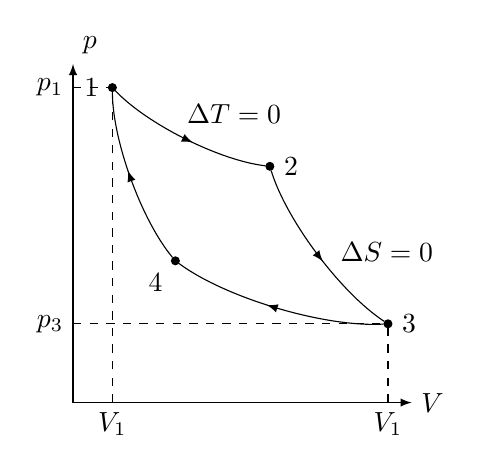
\begin{tikzpicture}[
  > = latex,
  dot/.style = {draw,fill,circle,inner sep=1pt},
  arrow inside/.style = {postaction=decorate,decoration={markings,mark=at position .55 with \arrow{>}}}
  ]
  \draw[<->] (0,4.3) node[above right] {$p$} |- (4.3,0) node[right] {$V$};
  \node[dot,label={left:$1$}] (@1) at (0.5,4) {};
  \node[dot,label={right:$2$}] (@2) at (2.5,3) {};
  \node[dot,label={right:$3$}] (@3) at (4,1) {};
  \node[dot,label={below left:$4$}] (@4) at (1.3,1.8) {};

  \node[label={above right:$\Delta T = 0$}] at (1.2,3.3) {};
  \node[label={above right:$\Delta S = 0$}] at (3.15,1.54) {};

  \draw[arrow inside] (@1) to[looseness=.7,bend right=20] (@2);
  \draw[arrow inside] (@2) to[looseness=.7,bend right=20] (@3);
  \draw[arrow inside] (@3) to[looseness=.7,bend left=20] (@4);
  \draw[arrow inside] (@4) to[looseness=.7,bend left=20] (@1);
  \draw[dashed,thin] (0,4) node[left] {$p_1$} -- (0.5,4);
  \draw[dashed,thin] (0,1) node[left] {$p_3$} -- (4,1);
  \draw[dashed,thin] (0.5,0) node[below] {$V_1$} -- (0.5,4);
  \draw[dashed,thin] (4,0) node[below] {$V_1$} -- (4,1);
\end{tikzpicture}

\section{Gemische Idealer Gase}

\begin{align*}
	&\xi_i = \frac{m_i}{m}, \quad \psi_i = \frac{n_i}{n}, \quad p_i = \psi_ip \\
	&\xi_i = \frac{M_i n_i}{\sum_{k = 1}^{K} M_kn_k} = \frac{M_i}{M_G}\psi  \\
	& p_iV = m_iR_iT, \quad p_iV = n_iR_mT, \quad pV = mR_GT \\
	& \sum_{k = 1}^{K} p_k = p \\
	&R_G = \frac{1}{m} \sum_{k=1}^{K} m_kR_k = \sum_{k=1}^{K} \xi_k R_k \\
	&U_G = \sum_{k=1}^{K} U_k = \sum_{k=1}^{K} m_k u_k = \sum_{k=1}^{K} c_{vk}m_kT \leftarrow \text{$c_v$ = const}\\
	&H_G = \sum_{k=1}^{K} H_k = \sum_{k=1}^{K} m_k h_k = \sum_{k=1}^{K} c_{pk}m_kT \leftarrow \text{$c_p$ = const.}\\
	&c_{vG} = \sum_{k=1}^{K} c_{vk} \xi_k, \quad c_{pG} = \sum_{k=1}^{K} c_{pk}\xi_k \\
	&S_2-S_1 = R_m \left( n \ln n - \sum_{k=1}^{K} n_k \ln n_k \right)
\end{align*}

\begin{align*}
	\text{Adiabate Drosselung (ideal): } &h + \frac{c^2}{2} + gz = \text{const.} \\
	&dh = 0 \\
	\text{Adiabet Drosselung (real): } &\delta_h = \left(\frac{\partial T}{\partial p}\right)_{h}  = - \frac{v}{c_p}(1-\beta T) \\
\end{align*}
\pagebreak
\section{Nassdampf}

\begin{multicols}{2}

\begin{align*}
	& v = (1-x)v^{'} + xv{''} \\
	& v = v^{'} + (v^{''}-v^{'})x \\ \\
	& u = (1-x) u^{'} + xu^{''} \\
	& u = u^{'} + (u^{''}-u^{'})x \\ \\
	& h = (1-x) h^{'} + xh^{''} \\
	& h = h^{'} + (h^{''}-h^{'})x \\ \\
	& s = (1-x) s^{'} + xs^{''} \\
	& s = s^{'} + (s^{''}-s^{'})x \\ \\
	& r = h^{''} - h^{'} = T(s^{''}-s^{'}) \\
\end{align*}

\begin{align*}
	& T^{'} = T^{''} \\
	& p^{'} = p^{''} \\
	& g^{'} = g^{''} \\
	&dg^{'} = v^{'}dp^{'} - s^{'}dT^{'} \\
	&dg^{''} = v^{''} dp^{''} - s^{''} dT^{''} \\
	&dg^{'} = dg^{''} \\
	& \frac{dp}{dT} = \frac{s^{''} - s^{'}}{v^{''} - v^{'}} \\
	& \frac{dp}{dT} = \frac{1}{T}\frac{h^{''} - h^{'}}{v^{''} - v^{'}} \\
	& \frac{dp}{dT} = \frac{1}{T}\frac{r}{v^{''} -v^{'}} \\
\end{align*}
\end{multicols}

\section{Realer Stoff im Nassdampfgebiet}
\begin{align*}
	\text{Isobare} &\text{Zustandsänderung} \\
	&q_{12} = T(s_2 - s_1) = T\Big(s^{''} - s^{'}\Big)(x_2-x_1) \\
	&w_{V,12} = - \int_{1}^{2} p\; dv = -p(v_2-v_1) = -p\Big(v^{''} -v^{'}\Big)(x_2-x_1) \\
	\text{Isochore} &\text{Zustandsänderung} \\
	&q_{12} = u_2 - u_1 = u_2^{'} + x_2\Big(u_2^{''} - u_2^{'} \Big) - u_1^{'} - x_1\Big(u_1^{''} - u_1^{'}\Big) \\
	\text{Adiabate} &\text{Zustandsänderung} \\
	& w_{V,12} = u_2 - u_1 = u_2^{'} + x_2 \Big( u_2^{''} - u_2^{'} \Big) - u_1^{'} - x_1\Big(u_1^{''} - u_1^{'}\Big) \\
\end{align*}

Entropieänderung wärend des Mischvorgangs
\begin{equation}
	S_2-S_2 = R_m \left ( n \ln n - \sum_{i}^{} n_i \ln n_i \right )
\end{equation}
\section{Maximale Arbeit und Exergie}

\begin{multline}
	-\dot{W}_{ex} = - (\dot{W}_t)_{rev} = -\frac{d}{dt} \left( U + m\left ( \frac{c^2}{2}+ gz \right) + p_uV - T_uS \right) \\  +  \sum_{j=1}^{K} \left(\dot{m}_j \left(h + \frac{c^2}{2} + gz -T_s \right) \right) + \sum_{l=1}^{K} \left( 1 - \frac{T_u}{T}\right) \dot{Q}_l 
\end{multline}

Die Exergie der Enthalpie (offens, stationäres System)
\begin{equation}
	-\dot{W}_{ex,1u} = \dot{m}(h_1 - h_u -T_u(s_1 - s_u))
\end{equation}
Die Exergie der inneren Energie (geschlossenes, instationäres System)
\begin{align}
	- \dot{W}_{ex} &= - \frac{d}{dt}(U + p_uV -T_uS) \\
	-\dot{W}_{ex,1u} &= U_1 - U_u -p_u(V_1 - V_u) - T_u(S_1 - S_u)
\end{align}
Die Exergie der Wärme (geschlossenes, stationäres System)
\begin{equation}
	- \dot{W}_{ex} = \left(1 - \frac{T_u}{T_1} \right) \dot{Q}_1 = \eta_{th,C} \dot{Q}_1 \\
\end{equation}

\section{Wärmekapazität}

\begin{align*}
	\text{Translatorisch: }  &C_v = \frac{3}{2} R_m  \\
	 \text{Rotatorisch: }  &C_v = n \cdot \frac{1}{2} R_m \\
	 n = \text{ Anzahl der Rotator} & \text{ischen Freiheitsgrade} \\
\end{align*}


\includepdf[pages=210]{/home/jonas/tu/thermo/2016_Book_ThermodynamikKompakt.pdf}
\includepdf[pages=211]{/home/jonas/tu/thermo/2016_Book_ThermodynamikKompakt.pdf}
%\includepdf[pages=201-211]{/home/jonas/tu/thermo/2016_Book_ThermodynamikKompakt.pdf}
%\includepdf[pages=213-216]{/home/jonas/tu/thermo/2016_Book_ThermodynamikKompakt.pdf}

\end{document}

%\begin{tabular}{l|l|l|l|l|l}
%	 & Isothermo  & Isobare  & Isochore  & reversibel Adiabat  & Polytrope \\ \hline
%	konstant:  & T  & p  & v  & $\delta q=0$  & $pv^n$  \\ \hline
%	 & -  & -  & -  & $p_1 v_1^{\kappa} = p_2 v_2^{\kappa}$  & $v_1^{n} = p_2 v_2^{n}$  \\ \hline
%	 & $p_1 p_2 = p_2 v_2$  & $\frac{v_1}{v_2} = \frac{T_1}{T_2}$  & $\frac{p_1}{T_1} = \frac{p_2}{T_2}$  & $T_1 v_1^{\kappa - 1} = T_2 v_2^{\kappa -1}$   & $T_1 v_1^{n - 1} = T_2 v_2^{n -1}$  \\ \hline
%	 & -  & -  & -  & $\frac{T_1^{\frac{\kappa}{\kappa -1}}}{p_1} = \frac{T_2^{\frac{\kappa}{\kappa -1}}}{p_2}$  & $\frac{T_1^{\frac{n}{n -1}}}{p_1} = \frac{T_2^{\frac{n}{n -1}}}{p_2}$  \\ \hline
%	p,v & $p = \frac{p_1 v_1}{v}$  & $p = p_1$  & $v = v_1$  & $p = \frac{p_1 v_1^{\kappa}}{v^{\kappa}}$  &  $p = \frac{p_1 v_1^{n}}{v^{n}}$ \\ \hline
%	p,T & $p = \frac{p_1 v_1}{v}$  & $p = p_1$  & $p = \frac{p_1}{T_1}T$  & $p = \frac{p_1}{T_1^{\frac{\kappa}{\kappa -1}}} T^{\frac{\kappa}{\kappa -1}}$  &  $p = \frac{p_1}{T_1^{\frac{n}{n -1}}} T^{\frac{n}{n -1}}$\\ \hline
%	v,T  & $T = T_1$  & $v = \frac{v_1}{T_1}T$  & $v = v_1 $ & $T = \frac{T_1 v_1^{\kappa - 1}}{v^{\kappa - 1}}$  & $T = \frac{T_1v_1^{n-1}}{v^{n-1}}  $\\ \hline
%	$w_{V,12}$  & $w_{V,12} = -q_{12}$ & $w_{V,12} = -p_1(v_2 - v_1)$  & $w_{V,12} = 0$  & $w_{V,12} = \frac{p_1 v_1}{k - 1}((\frac{v_1}{v_1}^{\kappa - 1} - 1)$  & $w_{V,12} = \frac{p_1 v_1}{n - 1}((\frac{v_1}{v_2}^{n-1} - 1)$ \\ \hline
%	&   &   &   &   &   \\ \hline
%	 &   &   &   &   &   \\ \hline
%	 &   &   &   &   &   \\
%\end{tabular}
%\\\\
